\documentclass[12pt]{article}

\usepackage[a4paper,margin=25mm]{geometry}
\usepackage{amsmath,amssymb}
\usepackage{booktabs}
\usepackage{graphicx}
\usepackage{microtype}
\usepackage{seqsplit}
\usepackage[numbers,sort&compress]{natbib}
\usepackage[hidelinks]{hyperref}

\newcommand{\logit}{\operatorname{logit}}
\newcommand{\E}{\mathbb{E}}

\title{Evidence-grounded belief revision as a prerequisite for\\
entropy-production measurements in decentralized LLM-agent networks}
\author{Anonymous working manuscript}
\date{17 August 2026}

\begin{document}
\maketitle

\begin{abstract}
Statistical-mechanical descriptions of language-model agents require more than
assigning binary spins to generated choices.  In particular, an empirical
transition kernel is meaningful only if communicated evidence measurably and
reproducibly changes an agent's local belief distribution.  We introduce a
controlled binary latent-state environment in which private and communicated
signals have explicit likelihoods, responses separate continuous belief from
action and commitment, and message effects are estimated with matched prompts
and cluster-level uncertainty.  A prospectively frozen experiment with
Qwen2.5-7B-Instruct comprised 864 decisions in 48 independent matched
information clusters.  Delivered evidence caused a positive average signed
change in reported belief log odds, $0.1343$ (95\% cluster-bootstrap interval
$0.0915$--$0.1811$), with positive application-specific intervals in two
semantic framings.  Nevertheless, the response was nonmonotone in source
reliability, binary choices were strongly right-skewed, and reported
probabilities were poorly calibrated to repeated choices.  These failures
triggered a prospective stop before reciprocal or nonreciprocal network
trajectories were generated.  The result therefore does not estimate entropy
production in an LLM network.  Instead, it identifies continuous evidence
response, directional symmetry, calibration, and transition diversity as
necessary qualification conditions for defensible coarse-grained stochastic
thermodynamics of decentralized LLM agents.
\end{abstract}

\section{Introduction}

Heat-bath dynamics, strategic logit response, and stochastic thermodynamics
provide a natural mathematical language for interacting decision makers
\cite{glauber1963,blume1993,seifert2012}.  Directed interactions can generate
stationary probability currents and positive entropy production even when the
reciprocal limit admits a Gibbs distribution
\cite{schnakenberg1976,zhang2023,dicarlo2025}.  Large language models (LLMs),
however, introduce private context, hidden memory, linguistic framing, and an
elicitation layer between the latent policy and the recorded state.  A binary
answer that does not switch after a message is consequently ambiguous: the
message may have been ignored, may have caused a subthreshold probability
update, or may have been overwhelmed by an option bias.

Recent work has begun to quantify collective alignment and conformity in LLM
populations \cite{han2026,denobili2026,okawa2026}, while observable belief
revision is itself an active measurement problem \cite{farmer2026}.  These
studies do not remove the need to identify the local response kernel before
applying pathwise irreversibility estimators.  Under coarse graining, hidden
degrees of freedom can make an observed entropy-production estimate only a
lower bound or can invalidate a first-order Markov interpretation
\cite{kawaguchi2013,roldan2012,skinner2021}.

This work reports a prospective qualification study.  Its purpose was to open
a decentralized reciprocal/nonreciprocal LLM-network experiment only if an
LLM used likelihood-bearing messages with sufficient monotonicity and
transition diversity.  The qualification found an average continuous belief
effect but failed two frozen requirements.  We preserve that no-go outcome and
use it to specify the measurement boundary, rather than estimating a network
quantity from an inadequate empirical state.

\section{Statistical-mechanical reference and measurement boundary}

The immutable preceding study defined a coupled belief--action microstate
$x=(\mathbf b,\mathbf a)$ with $b_i,a_i\in\{-1,+1\}$ and reciprocal energy
\begin{equation}
 H(x)=-\frac{J_b}{2}\sum_{ij}A^{(c)}_{ij}b_i b_j
      -\frac{J_a}{2}\sum_{ij}A^{(d)}_{ij}a_i a_j
      -K\sum_i a_i b_i-\sum_i h_i b_i-\sum_i g_i a_i .
 \label{eq:hamiltonian}
\end{equation}
With symmetric couplings, a static environment, common decision temperature,
and asynchronous heat-bath updates, the finite-state process obeys detailed
balance with $\pi(x)\propto\exp[-H(x)/T]$.  Directed communication was
parameterized as a symmetric component plus controlled antisymmetric
perturbation.  For a transition kernel
$W_\alpha=W_0+\alpha V+O(\alpha^2)$ around the reversible reference, the
stationary probability current is first order in $\alpha$, while its affinity
is also first order.  Their product gives the quadratic leading entropy
production
\begin{equation}
 \sigma(\alpha)=\frac12\sum_{x,y}J_{xy}(\alpha)
 \log\frac{\pi_\alpha(x)W_\alpha(x,y)}
               {\pi_\alpha(y)W_\alpha(y,x)}
 =C\alpha^2+O(\alpha^3).
 \label{eq:epr}
\end{equation}
That identity is exact for the specified finite Markov reference up to the
stated perturbative order; it is not automatically an identity for LLM text
generation.

For LLM agents, the recorded state was intended to be
$s_i=(p_i,b_i,a_i,c_i,m_i)$: reported probability, derived belief, typed
action, commitment, and bounded memory.  A network entropy-production claim
would additionally require stationarity or a declared driven protocol,
adequate state closure, nondegenerate transition estimates, and bias controls.
V11 tests the prerequisite local evidence response before attempting those
conditions.

\section{Independent LLM-agent architecture}

Each agent has a persistent identity, private signal and probability,
independent bounded memory, typed action authority, commitment, inbox, and
outbox.  Delivered packets are the only route by which peer evidence enters a
context.  The scheduler chooses an update opportunity and validates a typed
tool; it does not select the reported probability, belief, action, commitment,
or send/abstain decision.  Evaluator-only latent state is excluded from prompts.
Counterfactual tests modify one private vault while checking byte-identical
peer state.

\begin{figure}[t]
  \centering
  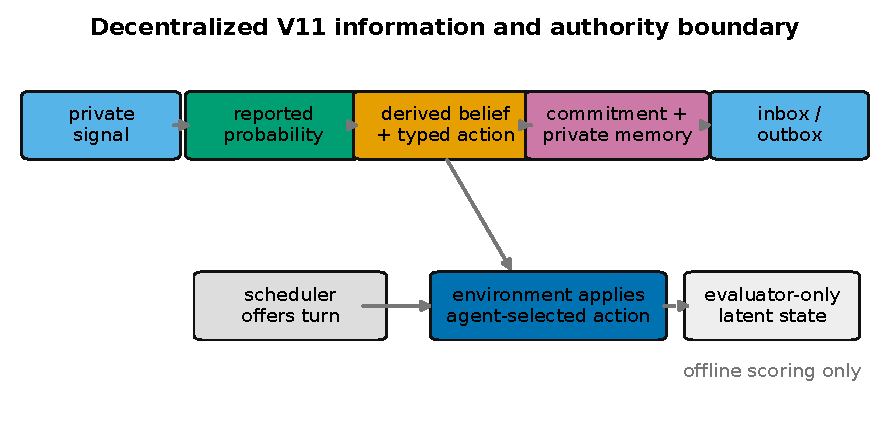
\includegraphics[width=\textwidth]{../../results/llm_agent_entropy_v11/figures/pdf/figure_01_architecture.pdf}
  \caption{V11 agent information and authority boundary.  The evaluator state
  is available only for offline scoring.}
  \label{fig:architecture}
\end{figure}

The primary model is \texttt{Qwen/Qwen2.5-7B-Instruct} \cite{qwen2024}.
Its pinned revision is
\texttt{\seqsplit{a09a35458c702b33eeacc393d103063234e8bc28}}; it is loaded with
NF4 double quantization and BF16 computation.  Sampling temperature is
$0.65$, top-$p$ is $0.90$, and at most one bounded JSON repair is allowed.
The inference sampling temperature is not interpreted as the effective
decision temperature in Eq.~\eqref{eq:hamiltonian}.

\section{Evidence-generating process}

Let $\theta\in\{L,R\}$ be a hidden evaluator state.  Agent $i$ observes a
conditionally independent signal $s_i$ with declared reliability $r_i$,
\begin{equation}
 P(s_i=\theta\mid\theta,r_i)=r_i,
 \qquad r_i\in\{0.55,0.65,0.75,0.85\}.
\end{equation}
The normative log-likelihood increment for an observation favouring $R$ is
$\log[r/(1-r)]$ and changes sign for an observation favouring $L$.  It is a
reference, not an instruction to emit a Bayesian posterior.  Packets include
source identity, observation, reliability, observation and delivery times,
freshness, domain, and deterministic wire serialization.

\begin{figure}[t]
  \centering
  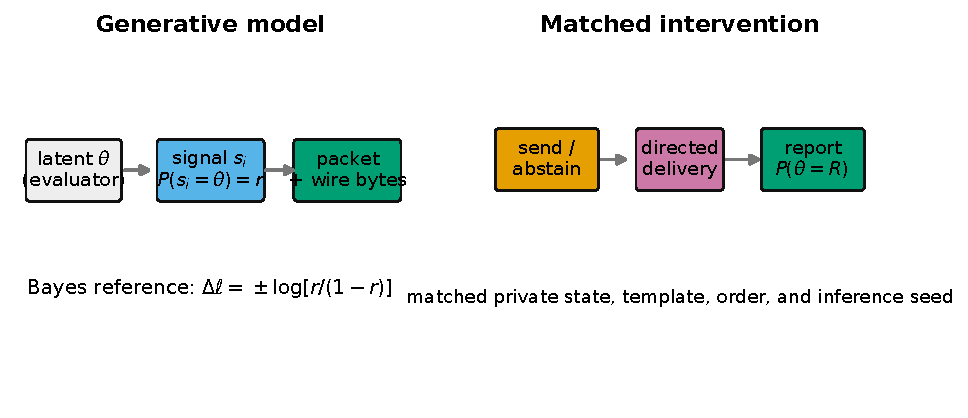
\includegraphics[width=\textwidth]{../../results/llm_agent_entropy_v11/figures/pdf/figure_02_evidence_process.pdf}
  \caption{Explicit signal model and matched evidence intervention.  Private
  state, prompt template, option order, and inference seed are held fixed.}
  \label{fig:evidence}
\end{figure}

Two application-neutral semantic frames instantiate the same probability
model: route viability and repair hypothesis.  Belief is elicited before
action and commitment.  The structured response contains
\texttt{probability\_right}$\in[0,1]$; $b_i$ is then derived using a frozen
$0.5$ threshold.  Repeated independent generations from identical information
states provide an empirical binary-choice frequency separate from the reported
probability.

\section{Prospective protocol and estimands}

An engineering pilot selected only interface and practical gate values.  The
decisive protocol was then frozen at SHA-256
\texttt{\seqsplit{7bd4082f9d085222e22d195e3ff603f0f76e27c36b347bfc4132fbb164a3d03f}}.
It specified 48 matched information clusters, three prompt paraphrases,
counterbalanced option order, two samples per condition, four reliabilities,
and 864 requests.  The independent unit is the information cluster, not the
generation or token.

For response $p_{ic}$ in condition $c$ and its no-message matched response
$p_{i0}$, the primary row effect is
\begin{equation}
 d_{ic}=q_c\{\logit(p_{ic})-\logit(p_{i0})\},
 \qquad q_c\in\{-1,+1\},
\end{equation}
oriented toward the evidence.  Cluster means are bootstrapped with 10,000
cluster resamples.  A direction-balanced placebo contrast removes a common
message-presence shift while retaining its magnitude as a diagnostic.

Progression required all components: first-pass and repaired validity, positive
directional and placebo-adjusted intervals with estimates at least $0.10$,
positive intervals in both frames, LLR-response slope at least $0.05$ with a
monotonic tolerance of $0.03$, bounded order/paraphrase effects, continuous
standard deviation at least $0.05$, each binary choice in at least 10\% of
valid responses, prompt isolation, and accepted agent-selected messages.
Failure locked the formal network stage.

\section{Qualification results}

There were 842 first-pass-valid responses, 21 repaired-valid responses, and one
invalid response after repair.  First-pass and final validity were 97.45\% and
99.88\%.  The primary signed effect was $0.1343$ (95\% cluster-bootstrap
interval $0.0915$--$0.1811$), and the placebo-adjusted estimate was $0.1343$
($0.0905$--$0.1816$).  Route viability yielded $0.1886$
($0.1164$--$0.2684$); repair hypothesis yielded $0.0799$
($0.0445$--$0.1197$).

\begin{figure}[t]
  \centering
  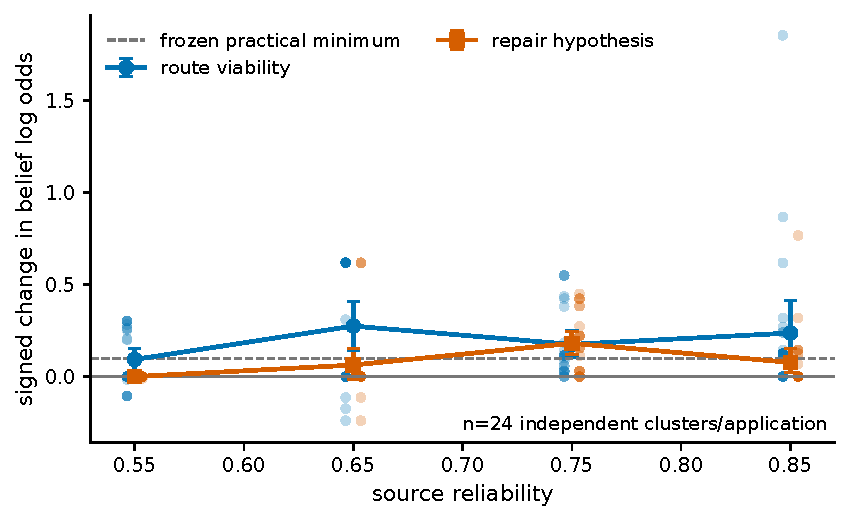
\includegraphics[width=0.88\textwidth]{../../results/llm_agent_entropy_v11/figures/pdf/figure_03_belief_response.pdf}
  \caption{Cluster-level signed log-odds response by source reliability.
  Points are independent cluster means; symbols show means and 95\% cluster
  bootstrap intervals.  The dashed line is the frozen practical minimum, not a
  fitted threshold.}
  \label{fig:response}
\end{figure}

The reliability-specific means were $0.0463$, $0.1686$, $0.1779$, and $0.1388$
at $r=0.55$, $0.65$, $0.75$, and $0.85$.  The fitted slope against normative
LLR was $0.04965$, below the frozen $0.05$ minimum; the decline at the highest
reliability exceeded tolerance.  The right-choice fraction was 0.9224, above
the frozen 0.90 ceiling.  Thus reliability monotonicity and transition
diversity failed, and the formal experiment did not run.

A post-qualification diagnostic, excluded from the progression decision,
localized substantial directional asymmetry.  Right-supporting packets had a
mean signed change of $0.5574$, while left-supporting packets had $-0.2939$.
The pooled positive effect therefore does not establish symmetric evidence
integration.

\subsection{Reported probability versus empirical choice}

Across 432 repeated-information cells, each with two independent samples, mean
reported $P(R)$ was 0.6697 whereas the empirical right-choice frequency was
0.9225.  The Brier score was 0.0968 and expected calibration error was 0.2955.
Two repetitions per cell are too few for a high-resolution calibration curve,
but the global discrepancy and choice degeneracy are sufficient to reject use
of the reports as calibrated transition probabilities.

\begin{figure}[t]
  \centering
  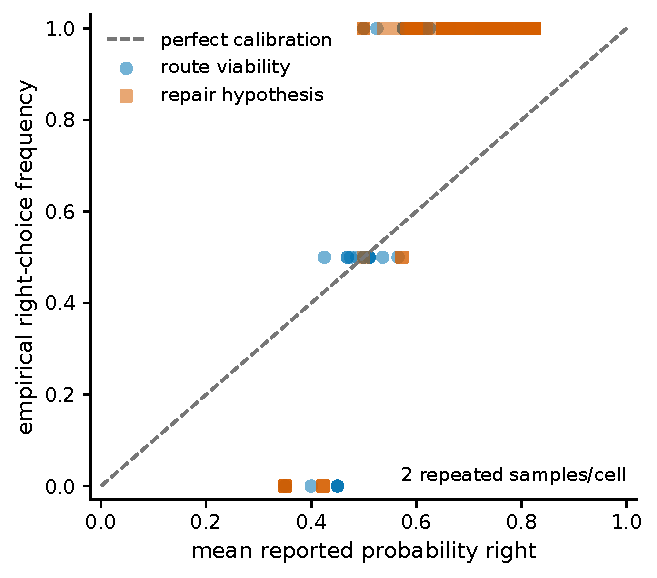
\includegraphics[width=0.70\textwidth]{../../results/llm_agent_entropy_v11/figures/pdf/figure_04_calibration.pdf}
  \caption{Reported probability and empirical repeated-choice frequency.  The
  figure is descriptive because each information cell has two repetitions.}
  \label{fig:calibration}
\end{figure}

\section{Why entropy production was not estimated}

Positive average message response is necessary but not sufficient for a
network estimator.  The frozen formal design would have compared reciprocal
and degree/traffic-matched directed networks, tested increasing history depth,
and estimated block time-reversal divergence with synthetic-chain bias
controls.  The qualification instead revealed (i) nonmonotone reliability
response, (ii) a nearly saturated right-choice process, (iii) poor calibration,
and (iv) post-gate direction asymmetry.  Estimating currents from that binary
state would conflate option bias with evidence flow and produce unstable
zero-count corrections.  Calling such a quantity exact entropy production
would be particularly misleading because hidden textual memory can violate
first-order Markov closure.

Consequently, V11 generated no reciprocal or nonreciprocal LLM trajectories,
no empirical stationary distribution, no transition-current entropy
production, and no Markov-adequacy estimate.  This is a prospective design
decision rather than absence of reporting.

\section{Modular-network anomaly inherited from V10}

An audit also resolved a V10 analytical-model anomaly without modifying its
frozen files.  The modular graph generator held within/between-community edge
probabilities fixed as $N$ grew, so mean degree increased while interaction
sums were not degree-normalized.  Local fields saturated, acceptance collapsed,
and trajectories froze.  Longer runs did not restore mixing; dividing the
adjacency by mean degree restored order-one acceptance and nonzero pathwise
estimates.  The effect was therefore a topology-construction and metastability
artifact, not universal modular scaling.  Any future formal LLM study must fix
mean degree or normalize coupling prospectively.

\section{Discussion}

The continuous endpoint repairs the central ambiguity of a binary switch test:
subthreshold message effects are now visible.  Yet a scalar probability emitted
in JSON is not automatically an empirical policy probability.  The V11 result
shows both sides.  Likelihood-bearing messages measurably changed the continuous
coordinate in two framings, but the response was biased and could not support a
diverse transition kernel.

The boundary has direct implications for statistical mechanics of LLM agents.
First, a recorded microstate must be operationally sufficient, not merely easy
to parse.  Second, reciprocal nulls require local response symmetry and
traffic-matched messaging in addition to symmetric graph support.  Third,
calibration should be estimated from repeated choice frequencies or constrained
token probabilities rather than assumed from narrated confidence.  Finally,
if finite memory materially predicts transitions after conditioning on the
nominal state, time-reversal divergence should be described as a coarse-grained
lower bound rather than full entropy production.

\section{Limitations}

The study uses one 7B instruction model, two simulated semantic framings, two
repetitions per information cell, and self-reported probabilities.  Paired
seeds reduce but cannot eliminate stochastic generation effects.  There are no
dynamic networks, no second model, no application performance outcomes, and no
human participants.  The post-gate direction analysis is exploratory.  The
inherited analytical heat-bath theory is exact for its finite model but does
not validate an LLM transition law.

\section{Conclusion}

Calibrated delivered evidence produced a detectable average continuous belief
shift, resolving the identifiability problem of the preceding binary test.
However, monotonicity and transition diversity failed prospectively, and
reported probabilities were not calibrated to empirical choices.  V11
therefore stops before measuring entropy production in an LLM-agent network.
Its positive contribution is a falsifiable qualification framework and a clear
measurement boundary for future statistical-mechanical studies of decentralized
LLM agents.

\section*{Data and software availability}

Source, frozen configuration, tests, aggregate tables, and vector figures are
in the V11 repository-facing package.  Raw prompts and completions are excluded
from Git and preserved under
\texttt{/workspace/ThermoAgent-v11-artifacts/}; directory tree checksums are in
\texttt{results/llm\_agent\_entropy\_v11/reproducibility/}.  The exact model
revision, environment versions, seeds, protocol hash, and reproduction commands
are recorded in the accompanying README.  No model weights are redistributed.

\appendix
\section{Frozen gate disposition}

\begin{table}[h]
\centering
\begin{tabular}{lll}
\toprule
Component & Result & Main diagnostic \\
\midrule
Structured validity & pass & 97.45\% first pass; 99.88\% repaired \\
Directional effect & pass & $0.1343$; CI excludes zero \\
Placebo-adjusted effect & pass & $0.1343$; CI excludes zero \\
Semantic replication & pass & positive interval in both frames \\
Reliability monotonicity & fail & slope 0.04965; high-$r$ decline \\
Transition diversity & fail & 92.24\% right choices \\
Order/paraphrase sensitivity & pass & within frozen bounds \\
Authority and prompt isolation & pass & deterministic tests and fingerprints \\
\bottomrule
\end{tabular}
\caption{Every component was required for progression.}
\end{table}

\section{Computational accounting}

The decisive qualification used 886 model calls, 559,895 prompt tokens, 76,620
generated tokens, and 1,536.064 seconds of measured generation latency on an
RTX 4090.  The retained pilot plus qualification used 1,017 calls and 0.4882
measured generation GPU-hours.  Three invalidated engineering pilots are
preserved externally; the earliest provider did not retain token usage for
responses invalid after repair, so all-pilot token totals are reported only as
documented lower bounds.

\bibliographystyle{unsrt}
\bibliography{references}

\end{document}
